\documentclass[11pt,letterpaper]{article}

%%%%%%%%%%%%%%%%%%%%%%%%%%%%%%%%%%%%%%%%%%%%%%%%%%%%%%%%%%%%%%%%%%%%%%%%%
\pagestyle{plain}                                                      %%
%%%%%%%%%% EXACT 1in MARGINS %%%%%%%                                   %%
\setlength{\textwidth}{6.5in}     %%                                   %%
\setlength{\oddsidemargin}{0in}   %% (It is recommended that you       %%
\setlength{\evensidemargin}{0in}  %%  not change these parameters,     %%
\setlength{\textheight}{8.5in}    %%  at the risk of having your       %%
\setlength{\topmargin}{0in}       %%  proposal dismissed on the basis  %%
\setlength{\headheight}{0in}      %%  of incorrect formatting!!!)      %%
\setlength{\headsep}{0in}         %%                                   %%
\setlength{\footskip}{.5in}       %%                                   %%
%%%%%%%%%%%%%%%%%%%%%%%%%%%%%%%%%%%%                                   %%
\newcommand{\required}[1]{\section*{\hfil #1\hfil}}                    %%
\renewcommand{\refname}{\hfil References Cited\hfil}                   %%
%\bibliographystyle{plain}                                             %%
%%%%%%%%%%%%%%%%%%%%%%%%%%%%%%%%%%%%%%%%%%%%%%%%%%%%%%%%%%%%%%%%%%%%%%%%%

%PUT YOUR MACROS HERE

\usepackage{amsmath}
\usepackage{amsfonts}
\usepackage{amssymb}
\usepackage{graphicx}
\usepackage{ulem}
\usepackage{placeins}

%\renewcommand{\thesection}{\Roman{section}} 
%\renewcommand{\thesubsection}{\thesection.\Roman{subsection}}

\title{Muon Physics}

\date{}

\author{Ian Hunt-Isaak}


\begin{document}


\maketitle
\begin{abstract}
We determined the detector lifetime of the TeachSpin Muon detector and investigated the effect that the number of bins used for histogramming that data has on the final result.
\end{abstract}
\section{Introduction}
Muon's were discovered back in the day with a sweet cloud chamber thing and conservation of momentum. Muon's are fundamental particles, they're like electrons but bigger. Are short lived. import in particle/nuclear physics CMS (compact MUON solenoid) 
\section{Background and Theory}
Muon's are generated as the result of cosmic ray's colliding with particles in the atmosphere. Muon's are very short lived and even with the very high speeds of atmospheric muons .99c almost all (~99 \%?) of the muons generated in the atmostphere should ahve decayed before reaching the Earth's surface. Yet by recording muon's at different altitudes we find that the fall off in number of muon's with altitude is not what we would expect given our classical picutre. The solution to this paradox comes from special relativity. The Muons' internal clocks \\ \\

Muon's come in two varieties, positively charged $\mu^+$ and negatively charged $\mu^-$. In free space we have that $\tau^+ = \tau^- = \tau_{free} = 2.1969811 \pm 0.0000022 × 10^{-6}$ (s) \cite{PDG}. However due to its negative charge the $\mu^-$ can interact with the orbitals of the carbon atoms in the detect, skirting the pauli exclusion principle as muon $\ne$ electron, which gives rise to another decay path for $\mu^-$ in the detector. The consequence of this is that in the detector we have $\tau^- < \tau^+$ and our observed decay time $\tau_{obs}$ will be a an average of $\tau^-$ and  $\tau^+$ weighted by the ratio of $\mu^+$ and $\mu^-$.
\begin{equation}
 \label{eq:t_obs}
     \tau_{obs} = \left(1+\frac{N^+}{N^-}\right)\frac{\tau^-\tau^+}{\tau^-+\tau^+}.
\end{equation}
For muons in the energy range of our detector we find this ratio to be 1.3\cite{ChargeRatio}. By rearranging Eq. \ref{eq:t_obs} we find the following the for the detector lifetime of $\mu^-$ for our detector:
\begin{equation}
\label{eq:t_minus}
\tau^- = \frac{\tau^+\tau_{obs}}{\left(1+\rho\right)\tau^+-\rho\tau_{obs}}.
\end{equation}

\section{Experimental Procedures}
%================================================================================
We turned on the Muon detector and waited for awhile.
Varied the threshold voltages
\section{Results}
\begin{figure}[h!]
  \centering
      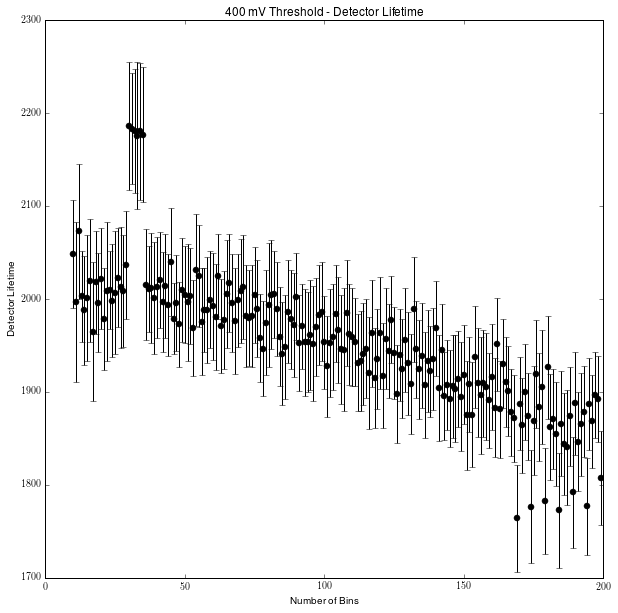
\includegraphics[scale=.7]{400mVDect.png}
      \caption{}
      \label{fig:400}
\end{figure}
\begin{figure}[h!]
  \centering
      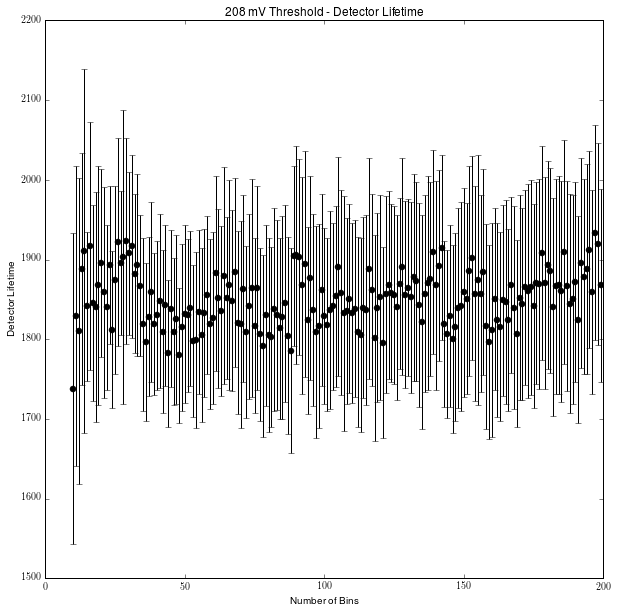
\includegraphics[scale=.7]{208mVDect.png}
      \caption{}
      \label{fig:208}
\end{figure}
\begin{figure}[h!]
  \centering
      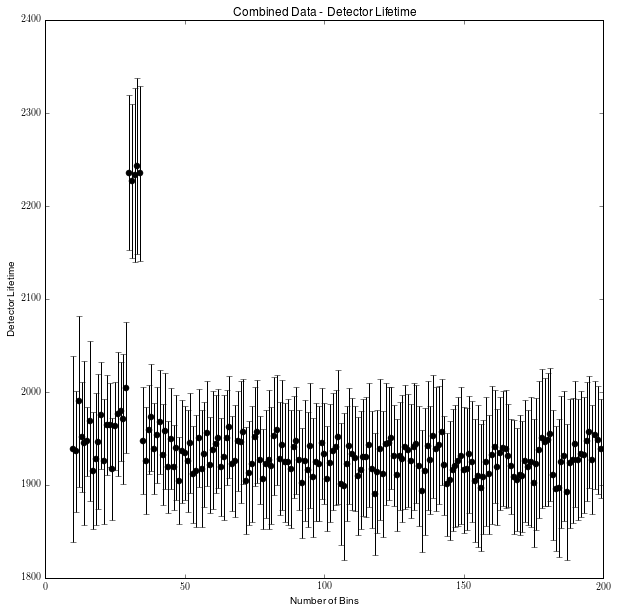
\includegraphics[scale=.7]{combinemVDect.png}
      \caption{}
      \label{fig:combine}
\end{figure}
\subsection{Uncertainty Budget}
The uncertainties for this experiment are determined by Poisson counting statistics and so for a histogram bin with N counts we have $\sigma_{counts}=\sqrt{N}$. As can be seen from \ref{fig:400} how the binning is chose introduces an error in the detector life time value. This may be in part due to the fact that with the 400 mV threshold and Nbins > 100 there were bins wiht 0 counts. In order to avoid division by zero in the least squares calculation (those points have zero error when calculating poisson statistics) those points were eliminated from the data used for the fit. This may in part account for the drop off of values with number of bins.
\begin{table}[!h]
	\begin{center} 
		\begin{tabular}{|c|c|c|c|} \hline 
			Source & Quantity&  Error in Quantity  & Propagated Error  \\ \hline \hline
			Model Error/Fitting Error& $T_1$ &  & 1.2 (ms)\\ \hline
			Model Error/Fitting Error& $T_2$ & & .55 (ms)\\ \hline
			Pulse Width&  & 5\% & .05 \%\\
			\hline
		\end{tabular}
        \caption{Uncertainty Budget for this work. The model for $T_1$ in particular may not be capable of fully describing the system. For more information see \ref{sec:ChiSq}.}
	\end{center}
\end{table}

\subsection{$\chi^2$ analysis}
The $\tilde{\chi}^2$ for the fit associated with each binning can also be plotted to see how this responds to binning. 
\begin{figure}[h!]
  \centering
      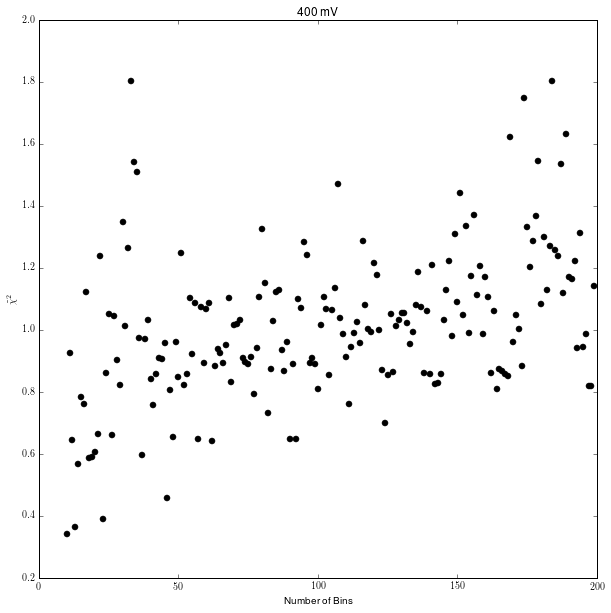
\includegraphics[scale=.7]{ChiSq_400.png}
      \caption{}
      \label{fig:400_Chi}
\end{figure}
\begin{figure}[h!]
  \centering
      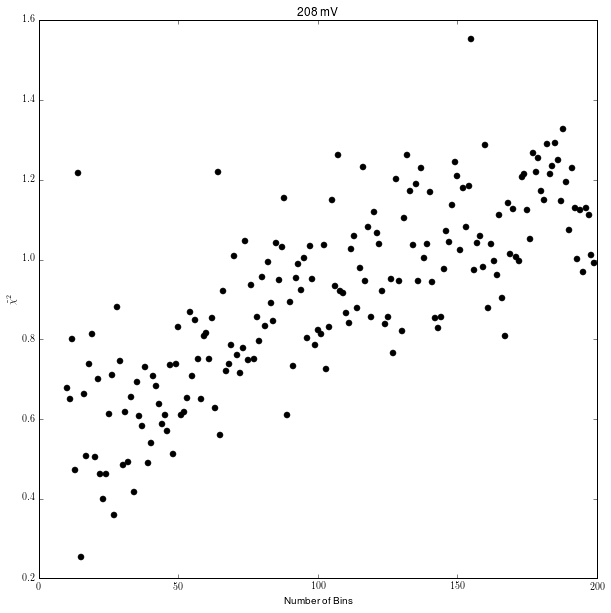
\includegraphics[scale=.7]{ChiSq_208.png}
      \caption{}
      \label{fig:208_Chi}
\end{figure}
\begin{table}[!h]

	\begin{center}
		\begin{tabular}{|c|c|c|c|c|} \hline
			Quantity & $\chi^2$&Deg Freedom&$\tilde{\chi}^2$  &  Probability \\ \hline \hline
			$T_1$ & 11.16 & 14 & .797 &  67 \%   \\ \hline
			$T_2$ & 18.55 & 15 & 1.23 & 14 \%   \\ \hline
		\end{tabular} \\
		\caption{Probabilities were determined from Ref. \cite{TaylorError}}
        \label{table:ChiSq}
	\end{center}
\end{table}

\section{Conclusions}
Muon Dector life time was determined to some level of accuracy. How you bin your histogram does actually matter. How to treat the data
\section{Acknowledgements}
Corina Miner was invaluable as a Lab Partner when performing this experiment.

\begin{thebibliography}{99}
\bibitem{PDG}  Particle Data GRoup!!
\bibitem{ChargeRatio} Conversation with jason Stalnaker



\end{thebibliography}
\end{document}